\documentclass[10pt,a4paper]{article}

% ---------------------------------------------------------------------------
% The phi^4 field as a second laboratory: the derivation, the estimator, the first
% measurements (E32, frozen), and the experiments in flight (E33, E34).
% Build: cd reports && tectonic -X compile field-laboratory-2026-10-01.tex
% Figures: python tools/make_report_field_figs.py (from outputs/E32, frozen).
% Every number here is traceable to outputs/E32 or to a registry entry.
% ---------------------------------------------------------------------------

\usepackage[T1]{fontenc}
\usepackage[utf8]{inputenc}
\usepackage{lmodern}
\usepackage[margin=1.85cm]{geometry}
\usepackage{microtype}
\usepackage{amsmath,amssymb,amsthm}
\usepackage{booktabs}
\usepackage{enumitem}
\usepackage{titlesec}
\usepackage{array}
\usepackage{graphicx}
\usepackage[hidelinks]{hyperref}

\newcommand{\Th}{\Theta}
\newcommand{\code}[1]{\texttt{\small #1}}
\newcommand{\st}[1]{\textbf{#1}}
\newcommand{\E}{\mathbb{E}}
\newcommand{\dd}{\,\mathrm{d}}
\newcommand{\Nn}{\mathcal{N}}
\theoremstyle{plain}
\newtheorem{proposition}{Proposition}
\newtheorem{lemma}[proposition]{Lemma}
\theoremstyle{remark}
\newtheorem{remark}[proposition]{Remark}
\titleformat{\section}{\large\bfseries}{\thesection}{0.6em}{}
\titlespacing*{\section}{0pt}{1.1em}{0.35em}
\titleformat{\subsection}{\normalsize\bfseries}{\thesubsection}{0.5em}{}
\titlespacing*{\subsection}{0pt}{0.8em}{0.25em}
\setlength{\parskip}{0.25em}
\setlength{\tabcolsep}{4.5pt}
\renewcommand{\arraystretch}{1.08}
\graphicspath{{figures/}}

\begin{document}

\begin{center}
{\Large\bfseries The $\phi^4$ field as a second laboratory}\\[0.25em]
{\normalsize The derivation, the estimator, the first measurements, and the experiments in flight}\\[0.35em]
{\footnotesize Jérôme's email of 1 October 2026 (after Marc) \textperiodcentered\ this report 1 October 2026 \textperiodcentered\ branch
\code{claude/phi4-field-2026-10-01} \textperiodcentered\ E32 frozen, E33 and E34 registered}
\end{center}

\vspace{-0.4em}

\section*{Summary}

Jérôme and Marc asked for a test of the estimator on Markov data from a physical model: spatial
snapshots of the one-dimensional stochastic Allen--Cahn ($\phi^4$) field, whose stationary law is a
nearest-neighbour Gibbs measure, with four arms tracked across temperature and lattice spacing (a
learned pair energy, the Gaussian closure, the window CNN, the exact score), and the suggestion that
with this concrete example the paper may be complete. Everything in this report was built, tested
and registered on 1 October; the deterministic part (E32) has run and is frozen; the learning
part (E33, eight cluster jobs) and the physics part (E34) are in flight.

\begin{enumerate}[leftmargin=1.4em,itemsep=0.15em]
\item \st{The chain is exact and in the package} (\S\ref{sec:chain}). Its kernel is a Gaussian step
  tilted by a function of the \emph{arrival} point, the column normaliser being the ground-state
  transform. The Gaussian AR(1) chain is the one member the two laboratories share
  (Proposition~\ref{prop:embed}); the paper's mixture kernel is misspecified here through a nonlinear
  drift, not through its innovation shape.
\item \st{The learned pair energy is a transition kernel} (\S\ref{sec:est}): concave M-step, the
  gradient is Boltzmann learning's positive phase minus a \emph{conditional} negative phase, no
  chain-wide partition function (Proposition~\ref{prop:boltz}). Two capacities, 7 and 25 parameters,
  the second the mixture's count.
\item \st{One thing in the email does not survive} (\S\ref{sec:closure}): moment projection of the
  messages is not a well-posed estimator on this chain, because the backward message is nearly flat.
  Measured: 42--100\,\% of a projected message's mass at the grid edge. The Gaussian-closure arm is
  therefore the covariance twin, which is what Proposition~1 of the paper proves projection
  computes on linear chains.
\item \st{E32} (\S\ref{sec:e32}): at matched correlation $\lambda_1/\lambda_0=0.85$ the linear floor
  is $0.269$ at $\Th=0.3$ against $0.168$ for the Laplace laboratory, and falls to $0.041$ at
  $\Th=2$; the operating grid is exact to $10^{-12}$; Theorem~2's gap ratio rises monotonically
  through $t_*$ to $0.73$--$0.94$ at $t=3$.
\item \st{E33 and E34} (\S\ref{sec:e33}): four kernel arms through exact BP, the window head and the
  transformer under both interfaces, the oracles; the physical statistics the consolidated note
  asks for; the clean-data interface. Nine predictions were registered before any confirmatory
  cell ran.
\end{enumerate}

Notation. $\Th$ is the physical temperature (the code and the cell names call it \code{T}), $h$ the lattice spacing,
$t$ the diffusion time of the channel $x_t=e^{-t}a+\sqrt{1-e^{-2t}}\,z$, $L$ the number of sites,
$M$ the number of training sequences, $N_g$ the grid size. The consolidated note's $\sigma$ is our
$\sqrt{1-e^{-2t}}/e^{-t}$.

\section{The chain}\label{sec:chain}

\subsection{From the SPDE to a Markov chain}

The equation $\partial_s\phi=\partial_x^2\phi-V'(\phi)+\sqrt{2\Th}\,\eta$ with $V(\phi)=(\phi^2-1)^2/4$
is the gradient flow of $H[\phi]=\int[\tfrac12(\partial_x\phi)^2+V(\phi)]\dd x$ at temperature
$\Th$; in one space dimension its stationary law is the Gibbs measure $\propto\exp(-H/\Th)$. On a
lattice of spacing $h$, $H_h(\phi)=\sum_i[(\phi_{i+1}-\phi_i)^2/2h+hV(\phi_i)]$, a nearest-neighbour
energy. A spatial snapshot is therefore a first-order Markov chain in the site index. Writing the
site terms symmetrically,
\begin{equation}
  \mathsf T(\phi,\phi')=D(\phi)\,G(\phi'-\phi)\,D(\phi'),\qquad
  D=e^{-hV/2\Th},\quad G(u)=e^{-u^2/2\Th h},
  \label{eq:T}
\end{equation}
is a symmetric, positive kernel, Hilbert--Schmidt for a confining $V$, with a simple largest
eigenvalue $\lambda_0$ and a positive eigenfunction $\psi_0$, $\int\psi_0^2=1$.

\begin{proposition}[ground-state transform]\label{prop:gs}
$K(\phi'\mid\phi)=\mathsf T(\phi,\phi')\psi_0(\phi')/(\lambda_0\psi_0(\phi))$ is a Markov kernel;
$\pi=\psi_0^2$ is invariant for it; and the chain is reversible, $\pi(\phi)K(\phi'\mid\phi)=\pi(\phi')K(\phi\mid\phi')$.
\end{proposition}
\begin{proof}
$\int K(\phi'\mid\phi)\dd\phi'=\int\mathsf T(\phi,\phi')\psi_0(\phi')\dd\phi'/(\lambda_0\psi_0(\phi))=1$ by the
eigen-equation. $\int\pi(\phi)K(\phi'\mid\phi)\dd\phi=\psi_0(\phi')\int\mathsf T(\phi,\phi')\psi_0(\phi)\dd\phi/\lambda_0=\psi_0(\phi')^2$
by symmetry of $\mathsf T$ and the eigen-equation again. $\pi(\phi)K(\phi'\mid\phi)=\psi_0(\phi)\mathsf T(\phi,\phi')\psi_0(\phi')/\lambda_0$
is symmetric in $(\phi,\phi')$.
\end{proof}
The infinite-volume Gibbs measure restricted to $L$ consecutive sites is this stationary chain,
$\pi(\phi_1)\prod K(\phi_{i+1}\mid\phi_i)$; that is what ``spatial snapshots of a stationary field''
means, and it is the law the data are drawn from. (A finite open chain with free ends is also
Markov but inhomogeneous within a correlation length of its ends; we do not use it.) The lag-$k$
covariance is $\sum_{n\ge1}(\lambda_n/\lambda_0)^k\langle\psi_0|\phi|\psi_n\rangle^2$, so $\rho_1:=\lambda_1/\lambda_0$
plays the role $\rho$ plays for the AR(1) family and the correlation length in sites is $1/\log(1/\rho_1)$.

\subsection{The tilted-walk identity}

\begin{proposition}[tilted walk]\label{prop:tilt}
With $g:=D\psi_0$,
\begin{equation}
  K(\phi'\mid\phi)=\frac{G(\phi'-\phi)\,g(\phi')}{Z(\phi)},\qquad
  Z(\phi)=\int G(\phi'-\phi)g(\phi')\dd\phi'=\frac{\lambda_0\psi_0(\phi)}{D(\phi)}.
  \label{eq:tilt}
\end{equation}
\end{proposition}
\begin{proof}
From \eqref{eq:T}, $\mathsf T(\phi,\phi')\psi_0(\phi')=D(\phi)G(\phi'-\phi)g(\phi')$, and the eigen-equation
reads $D(\phi)\int G(\phi'-\phi)g(\phi')\dd\phi'=\lambda_0\psi_0(\phi)$, which is the stated $Z$. Substituting in
Proposition~\ref{prop:gs}'s $K$ gives \eqref{eq:tilt}.
\end{proof}
So the kernel is a Gaussian random-walk step of variance $\Th h$, tilted by a positive function of
the arrival point and normalised per column: Jérôme's ``Gaussian increment tilted by
$\psi_0(\phi')e^{-hV(\phi')/\Th}/\psi_0(\phi)$'', with the normaliser made explicit. The point for the
estimator is that \emph{the column normaliser is the ground-state transform}: a family that
parametrises $\log g$ and normalises columns on the grid contains the truth exactly, and never needs
$\psi_0$ or $\lambda_0$.

\subsection{Where the two laboratories meet}

\begin{proposition}[Gaussian embedding]\label{prop:embed}
The Gaussian AR(1) kernel $\Nn(a';\rho a,q)$ with $0<\rho<1$ is the member of \eqref{eq:tilt} with
step variance $\gamma=q/\rho$ and $\log g(a')=-(1-\rho)a'^2/2q+\mathrm{const}$. No other kernel of
innovation form $p_\varepsilon(a'-\rho a)$, $\rho\neq0$, belongs to the family, and no other member of
the family has a state-independent innovation.
\end{proposition}
\begin{proof}
$\log\Nn(a';\rho a,q)=-a'^2/2q+\rho aa'/q-\rho^2a^2/2q+\mathrm{c}$ and $\log[G_\gamma(a'-a)g(a')]=-a'^2/2\gamma+aa'/\gamma-a^2/2\gamma+\log g(a')+\mathrm c$.
Matching the cross term gives $\gamma=q/\rho$; the $a'^2$ terms give $\log g(a')=-a'^2(1/q-\rho/q)/2$,
a Gaussian of variance $q/(1-\rho)=1+\rho$; the $a^2$ terms are absorbed by $Z(a)$. For the second
claim, $\partial_a\partial_{a'}\log K$ equals $1/\gamma$, a constant, for every member of \eqref{eq:tilt},
and equals $-\rho(\log p_\varepsilon)''(a'-\rho a)$ for an innovation kernel, which is constant iff
$\log p_\varepsilon$ is quadratic.
\end{proof}

\begin{remark}[the misspecification mechanism]
Expanding $\log g$ around $a$, $K(a'\mid a)\approx\Nn\!\big(a';\,a+\gamma(\log g)'(a),\,\gamma\big)$:
at fine $h$ the chain is the Euler step of $\dd a=\gamma(\log g)'(a)\dd s+\sqrt{2\gamma}\dd W$ with a
\emph{nonlinear} drift. The mixture-innovation kernel $\sum_c\pi_c\Nn(a'-\rho a;\mu_c,s_c^2)$ has a
linear drift and a state-independent innovation; it is misspecified here through the drift. That is
a different mechanism from every axis of the paper's misspecification study (global latent,
long-range coupling, AR(2), site-dependent $\rho$, heteroskedasticity), and E33's P1/P2 measure it.
\end{remark}

\subsection{Standardisation, cells}

Everything downstream assumes unit marginal variance, so the package exposes $a=\phi/s$,
$s^2=\mathrm{Var}_\pi(\phi)$ (the mean vanishes by symmetry); $K_a(a'\mid a)=sK_\phi(sa'\mid sa)$. The
$(\Th,h)$ map (Fig.~\ref{fig:spectrum}) gives the iso-correlation line $h^*(\Th)$ at $\rho_1=0.85$, the
laboratory's frozen correlation: it passes through $\Th=0.30$ at $h=1$. The temperature sweep sits
on that line, so the second laboratory is compared with the first at matched second-order
structure while the marginal kurtosis runs from $-1.35$ to $-0.46$; the refinement sweep halves $h$
twice from the base cell with $L\propto1/h$, so the physical length is fixed and the correlation
length in sites grows $6\to12\to24$ (Table~\ref{tab:cells}). The step width $\sqrt{\Th h}/s$ is at least
14 grid cells on every cell, so the usual resolution condition is met with room.

\begin{table}[h]\centering\footnotesize
\begin{tabular}{@{}l l l r r r r r@{}}
\toprule
cell & $\Th$ & $h$ & $L$ & $\rho_1$ & $\xi$ (sites) & $s$ & $\kappa_4(\pi)$ \\
\midrule
base      & 0.3 & 1      & 32  & 0.848 & 6.08  & 0.821 & $-1.352$ \\
T-sweep   & 0.5 & 0.419  & 32  & 0.850 & 6.15  & 0.766 & $-0.881$ \\
T-sweep   & 1.0 & 0.226  & 32  & 0.850 & 6.15  & 0.818 & $-0.588$ \\
T-sweep   & 2.0 & 0.150  & 32  & 0.850 & 6.15  & 0.950 & $-0.461$ \\
refine    & 0.3 & 0.5    & 64  & 0.917 & 11.47 & 0.805 & $-1.253$ \\
refine    & 0.3 & 0.25   & 128 & 0.957 & 22.48 & 0.800 & $-1.218$ \\
\bottomrule
\end{tabular}
\caption{The six confirmatory cells (\code{outputs/E32/cells.json}). $h^*$ solved by bisection to
$\rho_1=0.85\pm10^{-4}$; $\xi=1/\log(1/\rho_1)$.}
\label{tab:cells}
\end{table}

\begin{figure}[h]\centering
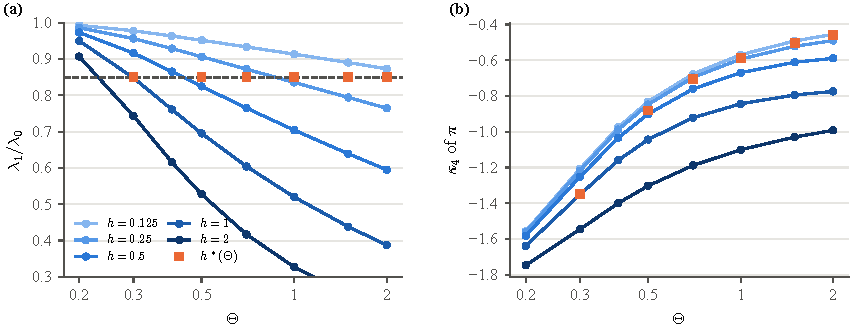
\includegraphics[width=\textwidth]{fig-field-spectrum.pdf}
\caption{The $(\Th,h)$ map of the chain. (a) $\lambda_1/\lambda_0$ against $\Th$ for five spacings; the dashed
line is the laboratory's $\rho=0.85$ and the squares are the solved $h^*(\Th)$. (b) Excess kurtosis
of the standardised marginal: the non-Gaussianity knob, platykurtic throughout (bimodal), from
$-1.75$ to $-0.46$.}
\label{fig:spectrum}
\end{figure}

\begin{figure}[h]\centering
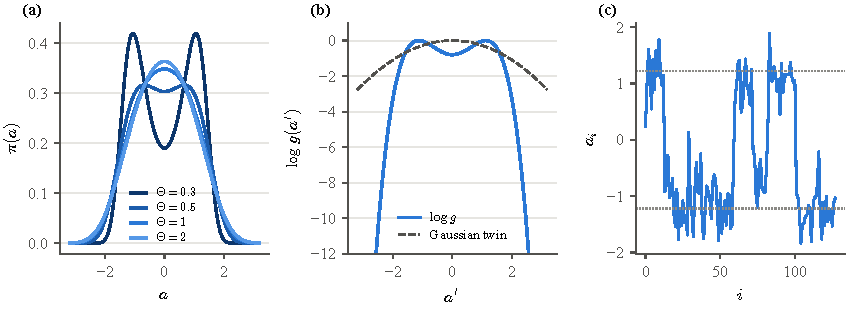
\includegraphics[width=\textwidth]{fig-field-chain.pdf}
\caption{The chain at the temperature cells. (a) The standardised stationary law $\pi=\psi_0^2$: two
wells at $\pm1/s$ merging as $\Th$ rises. (b) The arrival-point tilt $\log g$ at the base cell
against the quadratic tilt of its Gaussian twin (Proposition~\ref{prop:embed}): the truth is
bimodal and super-Gaussian, the twin is a parabola. (c) One exact sample of 128 sites at the base
cell; dotted lines at the wells. Domains of 5--25 sites separated by kinks.}
\label{fig:chain}
\end{figure}

\section{The estimator: the learned pair energy as a kernel}\label{sec:est}

The family is $K_\theta(a'\mid a)=\Nn(a';a,\gamma)\exp(B(a')\theta)/Z_\theta(a)$ with $B$ a linear basis
for $\log g$ (Legendre polynomials on $[-A,A]$, or cubic B-splines), the constant function omitted
(it is absorbed by $Z$), and $Z$ the column normaliser under the grid's trapezoid weights, exactly as
the MDN kernel is normalised. Parameters $(\log\gamma,\theta)$. In Jérôme's language, the pair energy is
$W_\theta(a,a')=(a'-a)^2/2\gamma-\log g_\theta(a')$ and the transfer-matrix normaliser is $Z_\theta(a)$.

\begin{lemma}[the M-step is concave in the tilt]
With $\Xi_{kj}$ the expected transition mass on $u_j\to u_k$ from the E-step and $N_j=\sum_k\Xi_{kj}$,
$Q(\theta)=\langle\Xi,\log K_\theta\rangle=\sum_k(\sum_j\Xi_{kj})B_k\theta-\sum_jN_j\log\sum_kw_k e^{B_k\theta+c_{kj}}$,
linear minus a sum of log-sum-exp functions, hence concave in $\theta$ at fixed $\gamma$; its gradient is
$\nabla_\theta Q=B^{\top}\!\sum_j\tilde\Xi_{\cdot j}$ with $\tilde\Xi_{kj}=\Xi_{kj}-N_jp_j(k)$, $p_j$ the model's
column distribution, and $\partial Q/\partial\log\gamma=\sum_{kj}\tilde\Xi_{kj}[(u_k-u_j)^2/2\gamma-\tfrac12]$.
\end{lemma}

\begin{proposition}[what Boltzmann learning becomes for a kernel]\label{prop:boltz}
By Fisher's identity the exact gradient of the noisy-data log-likelihood is $\langle\Xi,\nabla\log K_\theta\rangle$,
which for this family is
\[
  \nabla\mathcal L=\sum_j\Big[\sum_k\Xi_{kj}\,\nabla(-W_\theta(u_j,u_k))-N_j\,\E_{K_\theta(\cdot\mid u_j)}\!\big[\nabla(-W_\theta(u_j,\cdot))\big]\Big]:
\]
the positive phase is the posterior pair expectation (as in the note's \S16.2) and the negative
phase is the kernel's own \emph{conditional} expectation at each source state, weighted by the
posterior source mass. The undirected pair-energy model of the note's \S16 has instead the chain's
\emph{equilibrium} pair marginal as negative phase and a chain-wide $\log Z_\theta$. Both are exact
maximum likelihood for their model; the directed form needs no $Z_\theta$, its column normalisers are
the ground-state transform (Proposition~\ref{prop:tilt}), and it contains the field's kernel exactly.
\end{proposition}

Implementation (\code{src/markov\_score/tilted\_kernel.py}): L-BFGS-B on $(\log\gamma,\theta)$ with the
analytic gradient, warm-started, accepted only if $Q$ did not decrease (a rejected step returns the
receiver's parameters in a new object, so the checkpoint ladder stays honest); Fisher's identity
checked against finite differences of the evidence to $10^{-5}$; the Gaussian embedding recovered
on a Gaussian chain, and the field's kernel recovered from clean data with the spline basis
(\code{tests/test\_tilted\_kernel.py}). Two details earned by the first smoke run:

\begin{itemize}[leftmargin=1.4em,itemsep=0.1em]
\item \st{The tilt carries a fixed soft wall} $-(a/5)^{12}$ on the $(401,8)$ grid. The data occupy
  $|a|<4$, so the basis beyond that is constrained only through far columns' normalisers, and a free
  fit can raise the tilt at the grid edge and create a metastable pocket there, invisible to the
  likelihood but the place where the kernel's invariant law then puts mass. The wall is $0.002$ at
  $|a|=3$, $0.07$ at $4$ and $280$ at $8$, more than any coefficient within the optimiser's bounds can
  undo; the field's true tilt is already $-0.2a^4$ there.
\item \st{The initial law is the kernel's own invariant density}, by a direct eigensolve of the
  $401\times401$ operator (\code{em.fit\_em} takes a callable \code{log\_mu}): the model is a stationary
  chain, as the data are. The M-step maximises the edge term; any evidence decrease is recorded.
\end{itemize}

\section{What does not extend: Gaussian closure of the messages}\label{sec:closure}

The paper's Proposition~1 identifies moment-projected sum-product with the LMMSE of the covariance
twin, and its proof uses the linear transition. On the field chain the projected recursion is not a
well-posed estimator, for a reason that was found by the diagnostic, not anticipated.

\begin{proposition}[the backward message saturates]
Let $\log g(a')\le -c\,a'^4+C$ (a super-Gaussian tilt, $c>0$). Then $K(\cdot\mid a)$ concentrates, as
$|a|\to\infty$, near $a'_*(a)$ with $|a'_*|\sim(|a|/4c\gamma)^{1/3}$, and the backward message
$R(a)=\int K(a'\mid a)\ell(a')\dd a'=\E[\ell(a_{i+1})\mid a_i=a]$ is bounded and decays only as
$\exp(-c'|a|^{2/3})$.
\end{proposition}
\begin{proof}[Sketch]
The exponent $-(a'-a)^2/2\gamma-ca'^4$ is maximised where $(a-a')/\gamma=4ca'^3$, i.e.\ $a'_*\approx(a/4c\gamma)^{1/3}$
for large $|a|$, with curvature $\sim12ca'^2_*$, so $K(\cdot\mid a)$ is a sharpening Gaussian at $a'_*$ and
$R(a)\approx\ell(a'_*(a))$; for a Gaussian $\ell$ of width $\sqrt{\Delta}/\alpha$ this is $\exp(-\alpha^2(a'_*-x/\alpha)^2/2\Delta)$.
\end{proof}
So on a finite grid $R$ is nearly constant, and the Gaussian with its moments is close to flat: the
projection discards the backward information. Measured at $t=0.47$ on the $(401,8)$ grid, 28\,\% of
a projected message's mass sits in the outer 5\,\% of the grid; over E32's cells and levels the
maximum is 42\,\% at the base cell and 98--100\,\% at every other cell (Table~\ref{tab:ladder}). On
grids wide enough for the Gaussian and Laplace chains' backward messages (half-width 32 at $t=1$)
the projected recursion reproduces the LMMSE to $10^{-8}$ and $10^{-5}$, so this is a property of the
field, not of the implementation (\code{tests/test\_bp\_projected.py}).

Consequently the Gaussian-closure arm of the field chain is its covariance twin, the LMMSE of the
true covariance, by the identification Proposition~1 proves on linear chains; the projected
recursion is kept as the diagnostic and its edge mass is recorded. Jérôme's expectation that closure
``fails badly'' by smearing across domain walls is then measured by the linear floor, which is what
the floor has always measured, and it does: $0.269$ at the base cell. For the paper this is a
scope sentence on Proposition~1 and one sentence in the field section.

\section{E32: the laboratory before any learning}\label{sec:e32}

Deterministic, registered and predeclared, run on the laptop at commit \code{9b1c940}, frozen
(\code{outputs/E32}, 9 files). Three predictions were registered first.

\begin{table}[h]\centering\footnotesize
\begin{tabular}{@{}l r r r r r@{}}
\toprule
cell & linear floor & isotropic & projected (diag.) & edge mass & grid error \\
\midrule
$\Th=0.3$, $h=1$, $L=32$       & 0.269 & 0.674 & 0.262 & 0.42 & $9.6\times10^{-15}$ \\
$\Th=0.5$, $h^*$, $L=32$       & 0.115 & 0.658 & 0.278 & 1.00 & $1.3\times10^{-12}$ \\
$\Th=1$, $h^*$, $L=32$         & 0.058 & 0.657 & 0.208 & 0.99 & $1.3\times10^{-15}$ \\
$\Th=2$, $h^*$, $L=32$         & 0.041 & 0.656 & 0.169 & 0.98 & $1.6\times10^{-15}$ \\
$\Th=0.3$, $h=0.5$, $L=64$     & 0.162 & 0.714 & 0.291 & 1.00 & $2.3\times10^{-15}$ \\
$\Th=0.3$, $h=0.25$, $L=128$   & 0.098 & 0.750 & 0.529 & 1.00 & $1.1\times10^{-15}$ \\
\bottomrule
\end{tabular}
\caption{E32 ladder, pooled relative score error over the twelve-level schedule (mean of two
replicates of 512 chains), the projected recursion's largest edge mass over levels, and the worst
relative error of the $(401,8)$ exact score against $(1601,8)$ over levels. For scale: the Laplace
laboratory's floor at $\rho=0.85$ is $0.168$ and E14b's bimodal chain's $0.082$.}
\label{tab:ladder}
\end{table}

\begin{figure}[h]\centering
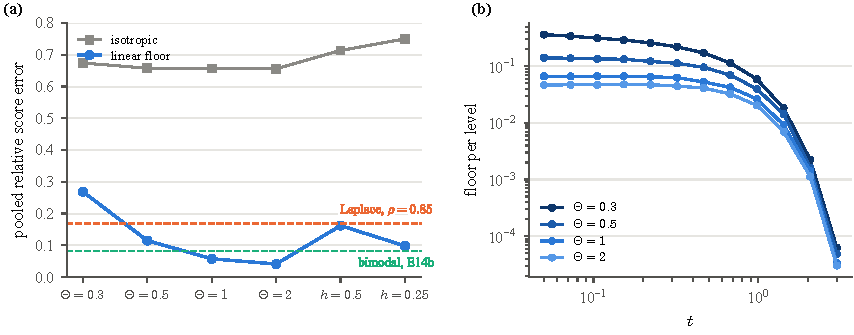
\includegraphics[width=\textwidth]{fig-field-ladder.pdf}
\caption{(a) The linear floor and the isotropic map across the six cells; dashed references are the
laboratory's Laplace floor and E14b's bimodal floor at the same correlation. (b) The floor per
level at the four temperature cells: the field's second-order deficit lives at low $t$ and is
largest where the wells are deepest.}
\label{fig:ladder}
\end{figure}

\begin{figure}[h]\centering
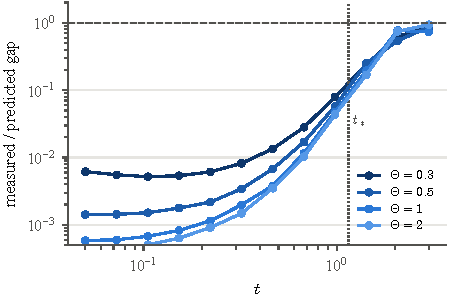
\includegraphics[width=0.52\textwidth]{fig-field-theory.pdf}
\caption{Theorem~2 on the second laboratory: $\E\|S-S^{\mathrm G}\|^2$ from tree-exact BP against the
linear floor, divided by $\tfrac16\|\kappa_4\|_F^2e^{-8t}$ with $\kappa_4$ from transfer-matrix
four-point functions, at the four temperature cells; $t_*=\tfrac12\log\lambda_{\max}(\Sigma_0)=1.15$.}
\label{fig:theory}
\end{figure}

\st{P1, the grid: confirmed far inside its bound.} The $(401,8)$ exact score agrees with the
$(1601,8)$ one to $10^{-12}$ relative or better on every cell and level, against a declared
tolerance of $10^{-3}$. The field kernel is smooth, so the trapezoid rule is spectrally accurate here,
unlike the Laplace chain's kink. The same holds for the eigensolve: halving the fine spacing or
widening the domain moves $\lambda_0$, $\rho_1$ and $s$ by less than $10^{-10}$.

\st{P2, the projection: confirmed.} The edge mass exceeds 10\,\% at some level of every cell
(Table~\ref{tab:ladder}); the closure arm is the covariance twin.

\st{P3, Theorem~2: consistent, not reached within the schedule.} The ratio rises monotonically
through $t_*$ and reads $0.85$, $0.87$, $0.73$, $0.94$ at $t=3$ on the four cells
(Fig.~\ref{fig:theory}). The AR(1) families reached the constant at $t=4$ with 8192 chains (E18);
this run stops at $t=3$ with 512, and the ratio at $t=2$ already moves by $0.1$ between the two
replicates. The constants are large, $C_4=\tfrac16\|\kappa_4\|_F^2=3882$, $2350$, $1261$, $838$ at
$\Th=0.3,0.5,1,2$ for $L=32$, which is why the gap is still $10^{-2}$--$10^{-1}$ of the score energy
at $t=1$. Extending the schedule to $t=4$ with 8192 chains is cheap and is the one addition E32 needs.

\st{The floor itself.} At the base cell the linear floor is $0.269$, well above the Laplace
laboratory's $0.168$ at the same correlation and more than three times E14b's bimodal chain's
$0.082$ (kurtosis $-0.72$): the field at $\Th=0.3$ carries more structure beyond second order than
any chain the paper has used, and the exact score has that much room above the floor. The floor
falls monotonically along the temperature sweep ($0.269\to0.041$), which is E33's P6, and along the
refinement cells ($0.269\to0.162\to0.098$), because at finer $h$ the per-step kernel is closer to
Gaussian while the chain is more correlated.

\section{E33 and E34: what is in flight}\label{sec:e33}

\subsection{E33, learning through noise}

On the six cells, under the registered protocol (sizes $M\in\{32,128,512,2048\}$, seeds $0$--$15$,
bundles keyed by tag, seed, cell and $M$, one noised view per sequence spread over the twelve
levels, validation 1024 and test 2048 chains per seed):

\begin{itemize}[leftmargin=1.4em,itemsep=0.1em]
\item kernel arms through exact BP, the same ladder to 1200 for every kernel, the kernel's own
  invariant law as initial law, both of E14's selection rules (held-out BP risk; held-out one-view
  evidence): \code{em\_mixture} ($C=8$, 25 parameters, misspecified), \code{em\_tilted\_poly} (Legendre
  degree 6, 7), \code{em\_tilted\_spline} (24 B-splines, 25), \code{em\_mdn} (E25/E30's neural kernel,
  1{,}516);
\item the window head and the transformer, re-screened per cell on development seeds and trained
  two ways, imported unchanged from E14: implicit score matching on the one-view bundle (the matched
  interface) and denoising score matching on clean targets with one fixed corruption (the
  network-favourable bracket), at $M\in\{2048,128\}$;
\item per (cell, seed): the linear floor, the isotropic map, the projected diagnostic.
\end{itemize}

Registered predictions. P1 the mixture keeps an asymptotic bias on every cell (above the spline in
16/16 seeds at $M=2048$, the gap not closing from 512 to 2048). P2 the learned pair energy beats the
mixture at every $M\ge128$ on every cell, the 7-parameter tilt within 20\,\% of the 25-parameter one
at $M=2048$. P3 the MDN improves relative to the mixture compared with E30 (mdn/mixture below 1.5
at $M=2048$): a state-dependent mean is what this chain needs. P4 no network reaches the spline at
any $M$ on any cell under either interface. P5 the window head's deficit grows along the refinement
cells while the spline's does not. P6 the floor at the base cell is above E14b's $0.082$ and falls
along the sweep (already visible in E32; the prediction stands as registered).

Jobs, deployment \code{9b1c940-20261001T084745Z}, submitted 08:55 UTC: oracles 678084
(\code{medium\_cpu}, running); kernels 678087--678090 (\code{defq}, four seed shards, each its own
directory); screen 678091 then nets 678092/678094 (\code{long\_gpuh200}, one H200 each; the A100
partition was in maintenance). The kernel shards are estimated at about eight hours each on 24
workers, the $L=128$ cells at $M=2048$ being the long pole; the network jobs at one to two days.

\subsection{E34, the physics and the clean-data interface}

The consolidated note (\S24.5, \S16.1) asks for physical statistics beside the score error and for
the clean-data baseline. E34 supplies them on E33's streams, so every row pairs with E33's:
\code{physics\_truth} (kink density per bond and per unit length, interior domain lengths, $C(r)$
against the spectral sum, kurtosis against the exact one, barrier mass, on 4096 exact chains per
cell; laptop); \code{clean} (the four kernel arms fitted by clean-data maximum likelihood on E33's
training chains, scored on E33's test bundles: the price of the channel per family; one cluster
job); \code{physics\_learned} (ancestral samples from every fitted E33 kernel at $M=2048$, started
from its own invariant law, the same statistics against the truth; after E33). Four predictions
registered; the quick smoke already shows the direction of two of them: on clean data at $M=32$ the
mixture sits at $0.27$ while the polynomial tilt reaches $0.04$, and samples from a fitted mixture
overshoot the truth's kink density ($0.21$ against $0.13$ per bond) while the spline's match it.

\section{Alignment with the consolidated note}

\begin{table}[h]\centering\footnotesize
\begin{tabular}{@{}p{4.3cm} p{12.2cm}@{}}
\toprule
the note asks for & where it is \\
\midrule
four arms across $\Th$, $h$, $\sigma$ & E33: learned pair energy (two capacities), closure = covariance twin (\S\ref{sec:closure}), window head, exact score; twelve levels $t$; six cells \\
exact transfer-matrix sampling & \code{field.py}: eigensolve on 2401 points, continuum rejection sampler and lattice inverse-CDF sampler, agreeing \\
score error, posterior-mean error & E33's estimand; the posterior-mean error is the same quantity per level up to $\alpha/\Delta$ \\
$C(r)$, $\xi$, kinks, domains, bimodality & E34 \code{physics\_truth} and \code{physics\_learned} \\
generated-sample quality & E34 \code{physics\_learned}; the direct sampler of E27 \\
runtime & E24x (uncontended reruns, in queue); the field adds nothing to BP's cost, which depends on $N_g$, $L$, $B$ only \\
clean-data learning (\S16.1) & E34 \code{clean} \\
symmetric $W_\theta$, reversibility & not enforced: the directed family contains the reversible truth; a symmetric restriction is a follow-up \\
Fourier BP for the SPDE (\S23) & not pursued: E24 found BP memory-bound (23.8\,\% of a sweep is the matmul), so a spectral step caps at $1.3\times$ \\
``minimal decisive experiment'' & E32 (floor across $\Th$, $h$) plus E33's window arm \\
figures-first (\S28) & figs.~5 and 6 of the note are E32/E33's; the summary figure is pending the E33 data \\
\bottomrule
\end{tabular}
\end{table}

\section{Questions for Jérôme and Marc}

\begin{enumerate}[leftmargin=1.4em,itemsep=0.15em]
\item The learned local law is implemented as a directed kernel with column normalisers
  (Proposition~\ref{prop:boltz}); the note's symmetric pair energy enforces reversibility and halves
  the parameters. Is there a reason to prefer the undirected form in the paper's framing, beyond
  physics taste? Both contain the truth; the directed one needs no chain-wide partition function.
\item Gaussian closure of the messages is not well-posed on the field (\S\ref{sec:closure}); the
  closure arm is the covariance twin. Does that match what Marc had in mind by ``Gaussian closure''
  for this benchmark, or did he mean the Kalman smoother of the linearised dynamics?
\item The temperature sweep is at matched $\lambda_1/\lambda_0=0.85$ rather than at fixed $h$, so that
  the field is compared with the AR(1) laboratory at matched second-order structure. Agreed, or
  would a fixed-$h$ sweep be more natural for the physics reading?
\item Theorem~2's ratio is still $0.75$--$0.95$ at $t=3$: the $\phi^4$ constants are large. Is it worth
  a sentence in the paper, or only the figure?
\end{enumerate}

\appendix
\section{Numerics}

\st{Eigensolve.} $A=W^{1/2}\mathsf TW^{1/2}$ on 2401 points of $[-12,12]$ (physical units), symmetric,
\code{scipy.linalg.eigh}; $\psi_n=W^{-1/2}v_n$. Components below $10^{-13}$ of the maximum are
eigensolver noise and are carried as $\log\psi_0=-\infty$ (stationary mass below $10^{-26}$); a kernel
column leaving such a state is the normalised $\mathsf T$ column. Spectral accuracy: $|\Delta\lambda_0|/\lambda_0<10^{-10}$,
$|\Delta\rho_1|<10^{-10}$ under halving the spacing and under widening the domain to $[-16,16]$.
Completeness: $\sum_nc_n^2=\mathrm{Var}_\pi(\phi)$ to $10^{-10}$.

\st{Samplers.} Continuum: propose $\phi'\sim\Nn(\phi,\Th h)$, accept with $g(\phi')/\max g$, $\log\psi_0$
by cubic spline on the resolved range; burn-in $\lceil\log(10^{-12})/\log\rho_1\rceil$ steps from
$\Nn(0,s^2)$. Lattice: inverse-CDF on the columns of the discretised kernel. Agreement in variance,
lag-one correlation and kurtosis within Monte Carlo error at 3000 chains.

\st{Fourth cumulant.} $\E[a_ia_ja_ka_l]$ for $i\le j\le k\le l$ equals
$\langle\psi_0|\,a\,R^{j-i}a\,R^{k-j}a\,R^{l-k}a\,|\psi_0\rangle$ with $R=\mathsf T/\lambda_0$, a triple sum over
the leading 256 modes with $\Phi_{nm}=\langle\psi_n|a|\psi_m\rangle$; $\kappa_4$ by Wick subtraction. The
diagonal reproduces the marginal excess kurtosis to $10^{-6}$.

\section{Tests}

33 new tests (59 pass in the files they live in, with the pre-existing ones): \code{test\_field.py} (14: stationarity, reversibility, column mass, the tilted-walk
identity, refinement, widening, completeness, two samplers, cumulant diagonal, BP as a denoiser, the
iso-correlation solver), \code{test\_tilted\_kernel.py} (7: the Gaussian embedding, Fisher's identity
by finite differences, M-step ascent and contract, clean MLE on the Gaussian chain and on the field,
EM through noise), \code{test\_bp\_projected.py} (6: identity and LMMSE on wide grids for the Gaussian
and Laplace chains, the truncation failure pinned, the field's near-flat backward message pinned),
\code{test\_stationary.py} (+2: eigensolve against power iteration; the wall), the kernel M-step
contract (+4). The fast suite is unchanged (178 passed).

\end{document}
